% !TEX TS-program = xelatex
% !TEX encoding = UTF-8 Unicode

% Tennessee Technological University
% ENGR1120-021 - GSET - Summer 2021
% Tristan Hill - June 02, 2021
% Module 1 - Introduction
% Lecture 1 - Creating a Program


\documentclass[fleqn]{beamer} % for presentation (has nav buttons at bottom)

\usepackage{/home/thill/Documents/lectures/cpp_workshop/modules/cpp_lectures}

\newcommand{\MNUM}{1\hspace{2mm}} % Module number
\newcommand{\TNUM}{---\hspace{2mm}} % Topic number - single topic for now
\newcommand{\moduletitle}{Creating a Program} % Titles and Stuff
%\newcommand{\topictitle}{---} 

\newcommand{\sectiontitleI}{Learning to Program} % More Titles and Stuff
\newcommand{\sectiontitleII}{Choosing a Language}
\newcommand{\sectiontitleIII}{C++ Program Structure}
\newcommand{\sectiontitleIV}{Compiling and Linking Source}
\newcommand{\sectiontitleV}{Up Next ...}

\setbeamercolor{title in head/foot}{fg=TTUgold} % this needs work...

\title{GSET - Programming with Mr. Hill}
\author{Tristan Hill\vspc \hspc Tennessee Technological University \hspc}
\date{Summer 2021}

\begin{document}

\lstset{language=MATLAB,basicstyle=\ttfamily\small,showstringspaces=false}

\frame{\titlepage \center\begin{framed}\Large \textbf{Module \MNUM - \moduletitle}\end{framed} \vspace{5mm}}

% Section 0 - Outline
\frame{
	
	\large \textbf{Module \MNUM - \moduletitle} \vspace{3mm}\\
	
	\begin{itemize}
	
		\item \hyperlink{sectionI}{\sectiontitleI} \vspc % Section I
		\item \hyperlink{sectionII}{\sectiontitleII} \vspc % Section II
		\item \hyperlink{sectionIII}{\sectiontitleIII} \vspc %Section III
		\item \hyperlink{sectionIV}{\sectiontitleIV} \vspc %Section IV	
		\item \hyperlink{sectionV}{\sectiontitleV} \vspc %Section V
	
	\end{itemize}

}

% Section I
\section{\sectiontitleI}

	% Section I - Frame I
	\begin{frame}[label=sectionI] \small
		\frametitle{\sectiontitleI}
		Programming is a skill that requires a lifetime of learning, and now is a great time to start.
		\begin{itemize}
			\item New Problems 
			\item New Languages
			\item New Hardware
		\end{itemize}
	\end{frame}

	% Section I - Frame II
	\begin{frame} \small
		\frametitle{\sectiontitleI}
		\underline{\large ---}	
		\begin{itemize}
			\item 
			
		\end{itemize}	
	\end{frame}

% Section II
\section{\sectiontitleII}

	% Section II - Frame I
	\begin{frame}[label=sectionII] \small
		\frametitle{\sectiontitleII}
		
		Question: How many programming languages exist today?
		\setbeamertemplate{itemize items}[triangle]
		\begin{multicols}{3}
		\begin{itemize}
			\item A.NET
			\item A-0 System \\
			 ...
			\item B
			\item Bash \\
			\item Fortran
			\item C
			\item C--
			\item C++
			... \\
			\item Python
			\item Java
			\item JavaScript
			\item MATLAB
			\item Tex
			... \\
		\end{itemize}
		\end{multicols}
		Answer: 
		
	\end{frame}

		% Section II - Frame II
	\begin{frame} \small
		\frametitle{\sectiontitleII}
		
		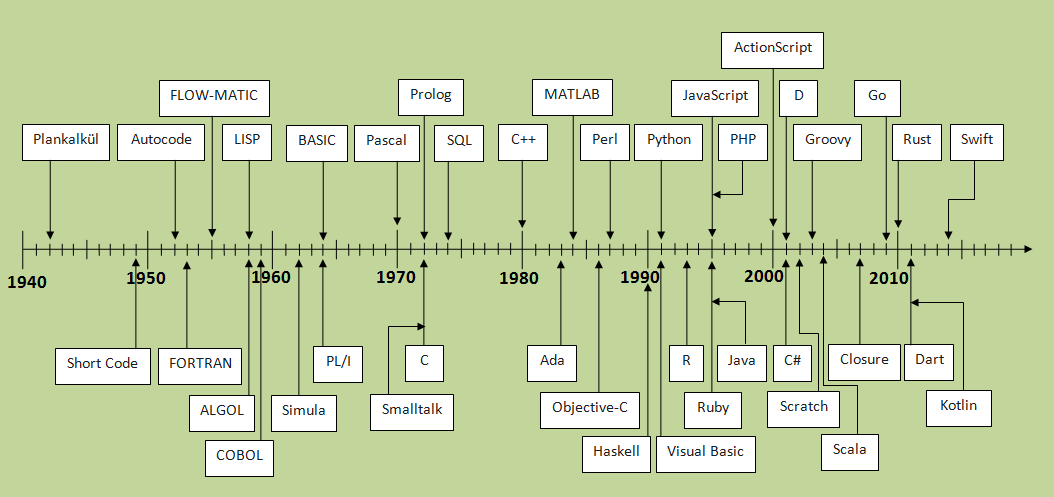
\includegraphics[scale=.4]{TimelineOfProgrammingLanguages.png} \\
		
		\tiny{Image: \href{https://javaconceptoftheday.com/history-of-programming-languages/}{Java Concept Of The Day}}
		
	\end{frame}	

	% Section II - Frame III
	\begin{frame} \small
		\frametitle{\sectiontitleII}
		
		Modern Programming Languages 
		\begin{itemize}
			\item C++
			\item Python
			\item JavaScript
		\end{itemize}
		
		Why is C++ important for scientists and engineers? 
		\begin{itemize}
			\item 
			\item
			\item
		\end{itemize}
	
	\end{frame}	

% Section III
\section{\sectiontitleIII}

	% Section III - Frame I
	\begin{frame}[label=sectionIII,containsverbatim] \small
		\frametitle{\sectiontitleIII}
		
		Look at the program from the previous tutorial.
		
		\begin{lstlisting}
		/*
		Hello World - June 3, 2021
		This is a comment
		*/
		
		#include <stdio.h>
		
		int main()
		{
			printf("Hello World");
		
			return 0;
		}
		
		\end{lstlisting}

	\end{frame}

% Section IV
\section{\sectiontitleIV}	
	% Section IV - Frame I
	\begin{frame}[label=sectionIV] \small
		\frametitle{\sectiontitleIV}    
		
		\underline{How does the computer run your code?} \vspace{5mm}\\
		
		\begin{tabular}{c|c} 
			\textbf{Compiled} \hspace{20mm} & \textbf{Interpreted} \hspace{20mm} \\ \hline
			 \hspace{20mm} &  \hspace{20mm} \\
			 \hspace{20mm} & \hspace{20mm} \\ 
			 \hspace{20mm} &  \hspace{20mm} \\
			 \hspace{20mm} & \hspace{20mm} \\
		
		\end{tabular}


	\end{frame}

	% Section IV - Frame I
	\begin{frame}[label=sectionIV] \small
		\frametitle{\sectiontitleIV}    
		
		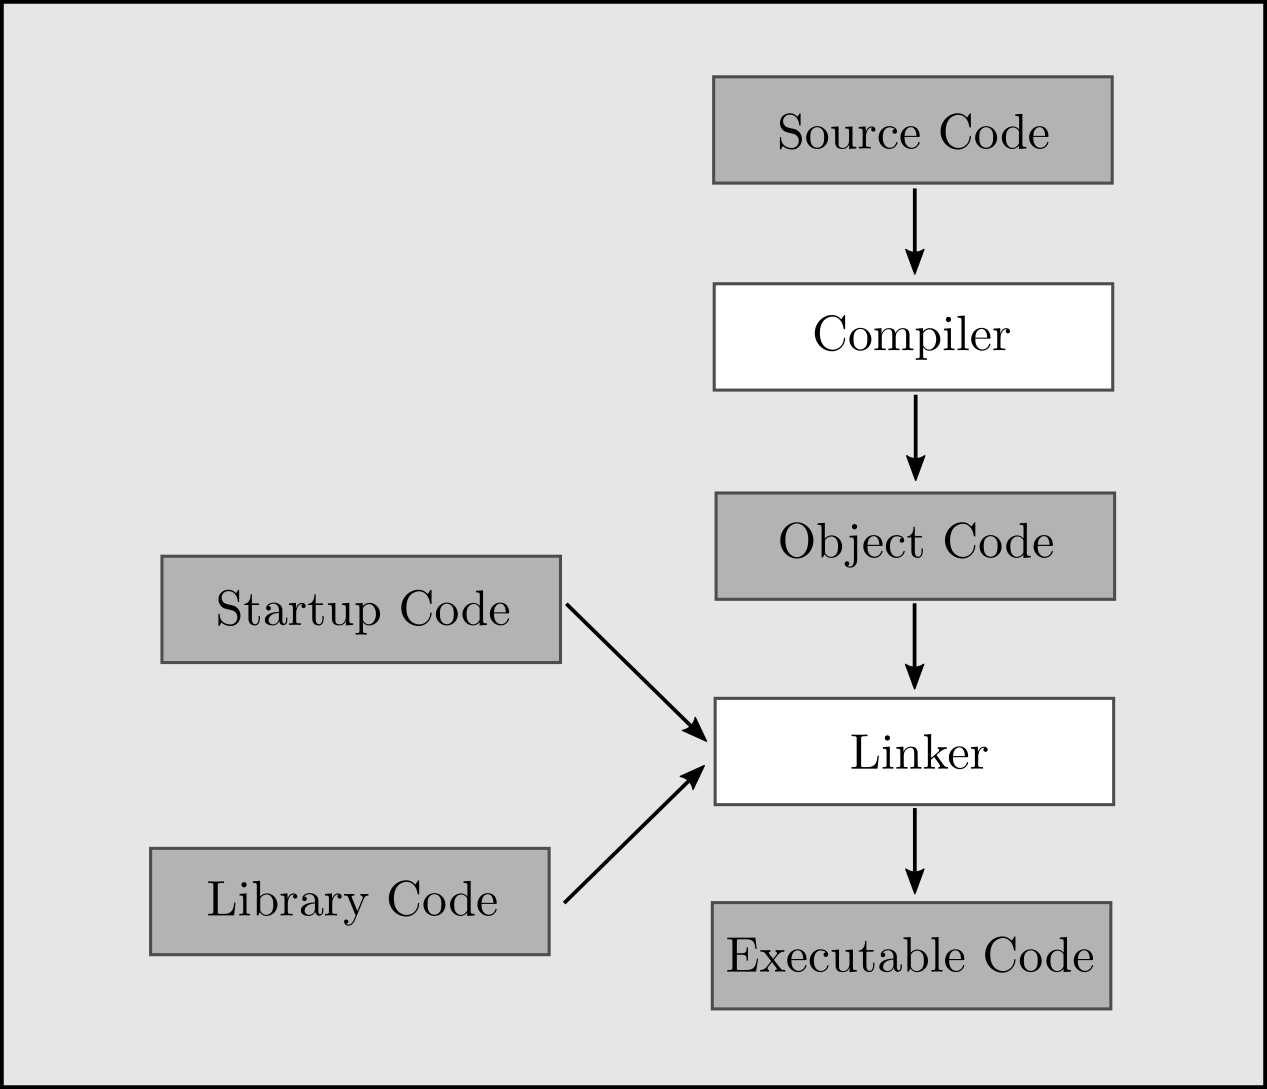
\includegraphics[scale=.2]{building_cpp_program.png} \\
		
		\tiny{Image: T.Hill from C++ Primer Plus by Stephen Prata}
		
	\end{frame}

% Section V
\section{\sectiontitleV}	
	% Section V - Frame I
	\begin{frame}[label=sectionV] \small
		\frametitle{\sectiontitleV}    
	
 			\setbeamertemplate{itemize items}[triangle]
            \begin{itemize}

                \item {\bf Next:} We are going to learn about Variables, Expressions and Assignment. \vspc

			
                
            \end{itemize}
	\end{frame}


\end{document}

